\documentclass[12pt]{article}
\usepackage[english]{babel}
\usepackage[margin=0.5in]{geometry}

\usepackage{amsmath,textcomp,blindtext,xcolor,multicol,color,comment,wrapfig,graphicx,amsthm}
\newtheoremstyle{colored}
  {\topsep}   % Space above
  {\topsep}   % Space below
  {}          % Body font
  {}          % Indent amount
  {\bfseries\color{red}} % Theorem head font - red color for 'def'
  {}          % Punctuation after theorem head
  {.5em}      % Space after theorem head
  {\thmnote{ \textbf{\color{red}#3}}} % Theorem head spec

\newtheoremstyle{subcolored}
  {\topsep}   % Space above
  {\topsep}   % Space below
  {}          % Body font
  {}          % Indent amount
  {\bfseries\color{blue}} % Theorem head font - blue color for 'subdef'
  {}          % Punctuation after theorem head
  {.5em}      % Space after theorem head
  {\thmnote{ \textbf{\color{blue}#3}}} % Theorem head spec

\theoremstyle{colored}
\newtheorem*{defn}{}

\theoremstyle{subcolored}
\newtheorem*{subdefn}{}


\begin{document}
\begin{center}
  {\LARGE \textbf{Sets}} \\
  
\end{center}
\begin{multicols}{2}


A well defined collection of objects/facts. The numbers constituting a set is called elements/members of
the set.

\begin{itemize}
    \item   Sets are generally represented by Capital letters and
    elements are denoted by small letters.\\
            eg: $A = \{\text{ Set of all natural numbers less than}\\10 \}, B =\{a,b,c,d,e,f,g\}$
    \item If $a$ is an element of a set $A$, we say that “ $a$ belongs to $A$” , we write $a \in A$. If '$b$' is not
    an element of a set $A$, we write $b \notin A$ and read “$b$ does not belong to $A$”. 

    eg: $5 \in A , 11 \notin A, a \in B , k \notin B$
\end{itemize}
\begin{subdefn}[Letter denoted by set:]
    \hfill \break
       $N$ -  Set of natural numbers \\
       $Z^+$ -  Set of all positive integers\\
       $Q$ -  Set of all rational numbers \\
       $R$ -  Set of all real numbers\\
       $C$ -  Set of all complex numbers\\
       $Z$ - Set of integers\\
       $Z^+$ - Set of -ve integers\\
      $ Q^+$ - Set of all positive rational numbers\\
       $R^+$ - Set of all positive real numbers\\
       $T $ - Set of irrational numbers

\end{subdefn}

\begin{defn}[\large Set Builder Form]
    \hfill \break
 In set builder form, the elements
of a set are described by their characterizing property

eg:
\begin{enumerate}
    \item[a)] $A = \{x: x \text{ is a natural number }<10\}$ OR  $A=\{x: x \in N,x<10 \}$
    \item[b)] $V = \{x : x \text{ is a vowel in English alphabet}\}$
    \item[c)] $A= \{x : x \text{ is a natural number which divides }\\42\}$
    \item[d)] $C= \{z : z \text{ is an odd natural number}\}$ 
\end{enumerate}

    
\end{defn}

\begin{subdefn}[Empty Set:]
    A set which does not contain any element is called the empty set or the
null set or the void set.

eg:\begin{enumerate}
    \item[a)] Let $A = \{x : 1 < x < 2, x$ is a natural number$\}$. 
    \item[b)] $C = \{x : x$ is an even prime number greater than $2\}$.
\end{enumerate}

\end{subdefn}

\begin{subdefn}[Finite and infinite Sets:]
    A set which is empty or consists of a definite number of elements is
called finite otherwise, the set is called infinite.

eg:
\begin{enumerate}
    \item[a)] Let W be the set of the days of the week. Then W is finite.
    \item[b)] Let G be the set of points on a line. Then G is infinite.
    \item[c)] Let S be the set of solutions of the equation $x^2 -16 = 0$. Then S is finite 
\end{enumerate}

It is not possible to write all the elements of an infinite set within
braces { } because the numbers of elements of such a set is not finite. So, we represent some infinite set in the roster form by writing a few elements which clearly indicate the
structure of the set followed ( or preceded ) by three dots.
For example, $\{1, 2, 3 . . .\}$ is the set of natural numbers, $\{1, 3, 5, 7, . . .\}$ is the set
of odd natural numbers, $\{. . .,-3, -2, -1, 0,1, 2 ,3, . . .\}$ is the set of integers.
\end{subdefn}

\begin{subdefn}[Equal Sets:]
    Two sets $A$ and $B$ are said to be equal if they have exactly the same
elements and we write $A = B$. Otherwise, the sets are said to be unequal and we write
$A \neq B$.
    
\end{subdefn}

\begin{defn}[\large Subsets]
    \hfill \break
    A set A is said to be a subset of a set B if every element of A is also an
element of B.In other words, $A \subset B$ if whenever $a \in A$, then $a \in B$. It is often convenient to
use the symbol $\Rightarrow$ which means implies. Using this symbol, we can write the definiton
of subset as follows:
eg:

$$A \subset B \text{ if } a \in A \Rightarrow a \in B$$

eg: \begin{enumerate}
    \item[a)] The set $Q$ of rational numbers is a subset of the set $R$ of real numbes, and
    we write $Q \subset R.$
    \item[b)]  Let $A = \{1, 3, 5\}$ and $B = \{x : x$ is an odd natural number less than $6\}$. Then
   $ A \subset B $and $B \subset A$ and hence $A = B$.
\end{enumerate}
\end{defn}

\begin{subdefn}[Proper Subset]
    Let A and B be two sets. If $A \subset B$ and $A \neq B$ , then A is called a proper subset
of B and B is called superset of A
    
\end{subdefn}
\begin{subdefn}[ Singleton set]
    If a set A has only one element, we call it a singleton set
   
\end{subdefn}
\begin{subdefn}[Subsets of set of real numbers]
    \begin{align*}
        N \subset Z \subset Q \subset R\\
        T \subset R \\
         N \not \subset T 
    \end{align*}

    
\end{subdefn}

\begin{subdefn}[Intervals as subsets of R]
    \hfill \break
    Let a and b be any two real numbers. If $a 
    < b$ , then\\
\begin{itemize}
    \item  $\{x : x \in R, a < x < b \}$ is known as open interval a,b. It is denoted as (a,b).
   \item  $\{x : x \in R, a \leq x \leq b \}$ is known as closed interval a,b. It is denoted as [a,b].
   \item  $\{x : x \in R, a \leq x < b \}$ is known as semi-closed interval a,b. It is denoted as [a,b).
   \item $\{x : x \in R, a < x \leq b \}$ is known as semi-open interval a,b. It is denoted as (a,b].
\end{itemize}

\begin{center}
    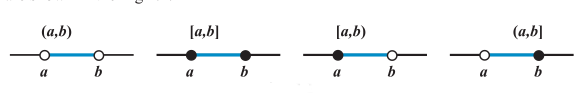
\includegraphics[scale=0.4]{set1.png}
\end{center}
The number (b – a) is called the length of any of the intervals (a, b), [a, b],
[a, b) or (a, b].
\end{subdefn}
\begin{subdefn}[Universal Set:]
    Usually, in a particular context, we have to deal with the elements and subsets of a
basic set which is relevant to that particular context. For example, while studying the
system of numbers, we are interested in the set of natural numbers and its subsets such
as the set of all prime numbers, the set of all even numbers, and so forth. This basic set
is called the “Universal Set”. The universal set is usually denoted by U, and all its
subsets by the letters A, B, C, etc.


note:

Number of subsets of a set with n elements = $2^n$
\end{subdefn}

\begin{defn}[\large Venn Diagrom]
    \hfill \break
    Venn Diagrom is a pictorial representation of sets. It consists of two closed figures - a rectangle for universal set and circles or
oval shaped circles for sets.

eg: 

\begin{center}
    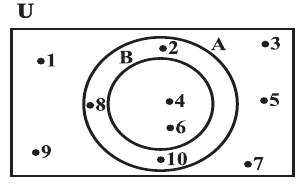
\includegraphics[scale=0.4]{set2.png}
\end{center}

U = \{1,2,3, ..., 10\} is the
universal set of which $A = \{2,4,6,8,10\}$ and $B = \{4, 6\}$ are subsets,
and also $B \subset A$.
    
\end{defn}

\begin{defn}[\large Union of Sets]
    \hfil \break
    Let A and B be any two sets. The union of A and B is the set
    which consists of all the elements of A and all the elements of B, the common elements
    being taken only once. The symbol $'\cup'$ is used to denote the union. Symbolically, we
    write $A \cup B$ and usually read as 'A union B'.
    $$A \cup B = \{ x : x \in A\, or\, x \in B \}$$
    \begin{center}
        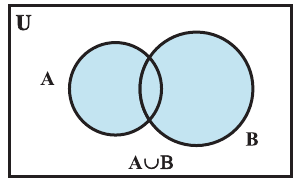
\includegraphics[scale=0.4]{set4.png}
    \end{center}

    eg:

    For  $A = \{ 2, 4, 6, 8\}$ and $B = \{ 6, 8, 10, 12\}$.
    We have $A \cup B$ = \{ 2, 4, 6, 8, 10, 12\}
\end{defn}

\begin{subdefn}[Some Properties of the Operation of Union]
    \hfill \break
    \begin{enumerate}
        \item[(i)] $A \cup B = B \cup A$  (Commutative Law)
        \item[(ii)] $(A \cup B)\cup C = A \cup (B \cup C)$ (Associative Law) 
        \item[(iii)] $A \cup \phi =A$ (Law of idntity)
        \item[(iv)] $A \cup A =A$ (Idempotent law) 
        \item[(v)] $U \cup A = U$ (Law of U)
    \end{enumerate}

\end{subdefn}

\begin{defn}[\large Intersection of Sets]
    \hfill \break
    The intersection of two sets A and B
is the set of all those elements which belong to both
A and B. Symbolically, we write
$$ A \cap B =\{x: x \in A\, and \, x \in B \}$$

\begin{center}
    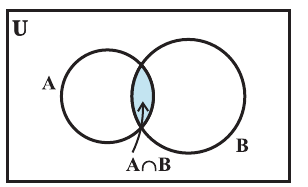
\includegraphics[scale=0.4]{set3.png}
\end{center}
    
In the previous example  6, 8 are the only elements which are common to both A and B.
Hence $A \cap B = \{ 6, 8 \}$
\end{defn}

\begin{subdefn}[Some Properties of the Operation of Intersection]
    \hfill \break
    \begin{enumerate}
        \item[(i)] $A \cap B = B \cap A$  (Commutative Law)
        \item[(ii)] $(A \cap B)\cap C = A \cap (B \cap C)$ (Associative Law) 
        \item[(iii)] $A \cap \phi =\phi$ (Law of idntity)
        \item[(iv)] $A \cap A =A$ (Idempotent law) 
        \item[(v)] $U \cap A = A$ (Law of U)
        \item[(vi)] $A \cap (B \cup C)= (A \cap B) \cup (A \cap C)$ (Distributive law)
    \end{enumerate}

    \begin{center}
        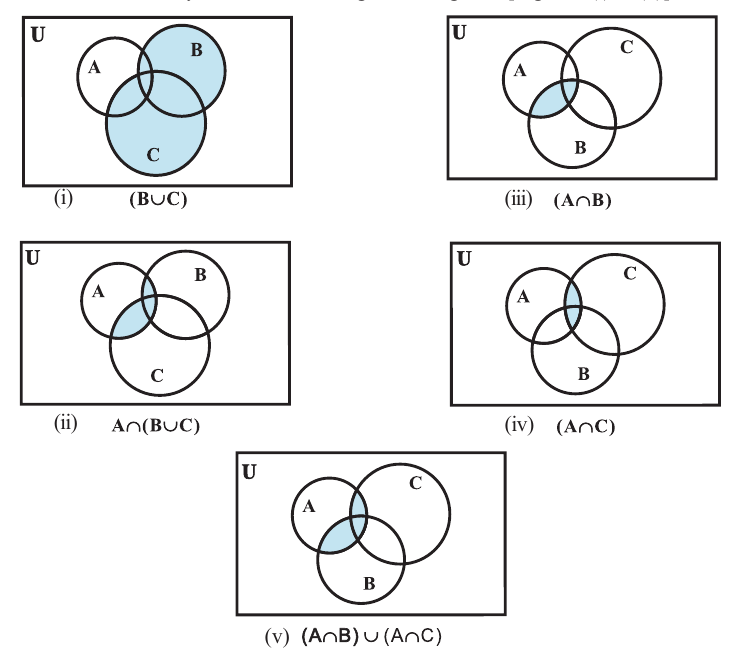
\includegraphics[scale=0.35]{set5.png}
    \end{center}

\end{subdefn}

\begin{defn}[\large Difference of sets ]
    \hfill \break
    The difference of the sets A and B in this order is the set
of elements which belong to A but not to B. Symbolically, we write A - B and read as
“A minus B”.

\begin{center}
    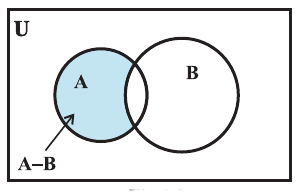
\includegraphics[scale=0.4]{set6.png}
\end{center}

In the previous example $A-B=\{2,4\}$
\end{defn}

\begin{defn}[\large Complement of a Set]
    \hfill \break 
    Let U be the universal set and A a subset of U. Then the complement of
A is the set of all elements of U which are not the elements of A.
$$A=\{x: x \in U\, and\, x \not \in A\}$$

\begin{center}
    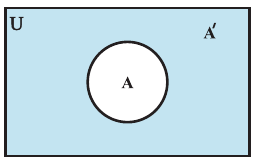
\includegraphics[scale=0.4]{set7.png}
\end{center}

\end{defn}

\begin{subdefn}[Some Properties of Complement Sets]
    \hfill \break
    \begin{enumerate}
        \item (Complement Laws) $A \cup A'=U$ ,  $A \cap A'= \phi$
        \item (De Morgan's Law) $(A \cup B)'= A' \cap B'$ , $(A \cap B)'= A' \cup B'$
        \item (Law of double complementation) $(A')'=A$
        \item  (Laws of empty set and universal set) $\phi ' = U$ , $U'=\phi$
    \end{enumerate} 
    
\end{subdefn}
\end{multicols}
 \end{document}

 